% Options for packages loaded elsewhere
% Options for packages loaded elsewhere
\PassOptionsToPackage{unicode}{hyperref}
\PassOptionsToPackage{hyphens}{url}
\PassOptionsToPackage{dvipsnames,svgnames,x11names}{xcolor}
%
\documentclass[
  spanish,
  11pt,
  a4paper,
  DIV=11,
  numbers=noendperiod]{scrartcl}
\usepackage{xcolor}
\usepackage{amsmath,amssymb}
\setcounter{secnumdepth}{5}
\usepackage{iftex}
\ifPDFTeX
  \usepackage[T1]{fontenc}
  \usepackage[utf8]{inputenc}
  \usepackage{textcomp} % provide euro and other symbols
\else % if luatex or xetex
  \usepackage{unicode-math} % this also loads fontspec
  \defaultfontfeatures{Scale=MatchLowercase}
  \defaultfontfeatures[\rmfamily]{Ligatures=TeX,Scale=1}
\fi
\usepackage{lmodern}
\ifPDFTeX\else
  % xetex/luatex font selection
\fi
% Use upquote if available, for straight quotes in verbatim environments
\IfFileExists{upquote.sty}{\usepackage{upquote}}{}
\IfFileExists{microtype.sty}{% use microtype if available
  \usepackage[]{microtype}
  \UseMicrotypeSet[protrusion]{basicmath} % disable protrusion for tt fonts
}{}
\makeatletter
\@ifundefined{KOMAClassName}{% if non-KOMA class
  \IfFileExists{parskip.sty}{%
    \usepackage{parskip}
  }{% else
    \setlength{\parindent}{0pt}
    \setlength{\parskip}{6pt plus 2pt minus 1pt}}
}{% if KOMA class
  \KOMAoptions{parskip=half}}
\makeatother
% Make \paragraph and \subparagraph free-standing
\makeatletter
\ifx\paragraph\undefined\else
  \let\oldparagraph\paragraph
  \renewcommand{\paragraph}{
    \@ifstar
      \xxxParagraphStar
      \xxxParagraphNoStar
  }
  \newcommand{\xxxParagraphStar}[1]{\oldparagraph*{#1}\mbox{}}
  \newcommand{\xxxParagraphNoStar}[1]{\oldparagraph{#1}\mbox{}}
\fi
\ifx\subparagraph\undefined\else
  \let\oldsubparagraph\subparagraph
  \renewcommand{\subparagraph}{
    \@ifstar
      \xxxSubParagraphStar
      \xxxSubParagraphNoStar
  }
  \newcommand{\xxxSubParagraphStar}[1]{\oldsubparagraph*{#1}\mbox{}}
  \newcommand{\xxxSubParagraphNoStar}[1]{\oldsubparagraph{#1}\mbox{}}
\fi
\makeatother

\usepackage{color}
\usepackage{fancyvrb}
\newcommand{\VerbBar}{|}
\newcommand{\VERB}{\Verb[commandchars=\\\{\}]}
\DefineVerbatimEnvironment{Highlighting}{Verbatim}{commandchars=\\\{\}}
% Add ',fontsize=\small' for more characters per line
\usepackage{framed}
\definecolor{shadecolor}{RGB}{243,245,250}
\newenvironment{Shaded}{\begin{snugshade}}{\end{snugshade}}
\newcommand{\AlertTok}[1]{\textcolor[rgb]{0.71,0.02,0.11}{\textbf{#1}}}
\newcommand{\AnnotationTok}[1]{\textcolor[rgb]{0.30,0.33,0.46}{\textit{#1}}}
\newcommand{\AttributeTok}[1]{\textcolor[rgb]{0.04,0.38,0.43}{#1}}
\newcommand{\BaseNTok}[1]{\textcolor[rgb]{0.55,0.27,0.02}{#1}}
\newcommand{\BuiltInTok}[1]{\textcolor[rgb]{0.04,0.38,0.43}{#1}}
\newcommand{\CharTok}[1]{\textcolor[rgb]{0.55,0.27,0.02}{#1}}
\newcommand{\CommentTok}[1]{\textcolor[rgb]{0.30,0.33,0.46}{\textit{#1}}}
\newcommand{\CommentVarTok}[1]{\textcolor[rgb]{0.30,0.33,0.46}{\textit{#1}}}
\newcommand{\ConstantTok}[1]{\textcolor[rgb]{0.55,0.27,0.02}{#1}}
\newcommand{\ControlFlowTok}[1]{\textcolor[rgb]{0.45,0.21,0.74}{#1}}
\newcommand{\DataTypeTok}[1]{\textcolor[rgb]{0.04,0.38,0.43}{#1}}
\newcommand{\DecValTok}[1]{\textcolor[rgb]{0.55,0.27,0.02}{#1}}
\newcommand{\DocumentationTok}[1]{\textcolor[rgb]{0.30,0.33,0.46}{\textit{#1}}}
\newcommand{\ErrorTok}[1]{\textcolor[rgb]{0.71,0.02,0.11}{\textbf{#1}}}
\newcommand{\ExtensionTok}[1]{\textcolor[rgb]{0.04,0.38,0.43}{#1}}
\newcommand{\FloatTok}[1]{\textcolor[rgb]{0.55,0.27,0.02}{#1}}
\newcommand{\FunctionTok}[1]{\textcolor[rgb]{0.04,0.38,0.43}{#1}}
\newcommand{\ImportTok}[1]{\textcolor[rgb]{0.45,0.21,0.74}{#1}}
\newcommand{\InformationTok}[1]{\textcolor[rgb]{0.71,0.02,0.11}{#1}}
\newcommand{\KeywordTok}[1]{\textcolor[rgb]{0.45,0.21,0.74}{#1}}
\newcommand{\NormalTok}[1]{\textcolor[rgb]{0.08,0.09,0.23}{#1}}
\newcommand{\OperatorTok}[1]{\textcolor[rgb]{0.08,0.09,0.23}{#1}}
\newcommand{\OtherTok}[1]{\textcolor[rgb]{0.08,0.09,0.23}{#1}}
\newcommand{\PreprocessorTok}[1]{\textcolor[rgb]{0.45,0.21,0.74}{#1}}
\newcommand{\RegionMarkerTok}[1]{\textcolor[rgb]{0.08,0.09,0.23}{#1}}
\newcommand{\SpecialCharTok}[1]{\textcolor[rgb]{0.55,0.27,0.02}{#1}}
\newcommand{\SpecialStringTok}[1]{\textcolor[rgb]{0.55,0.27,0.02}{#1}}
\newcommand{\StringTok}[1]{\textcolor[rgb]{0.55,0.27,0.02}{#1}}
\newcommand{\VariableTok}[1]{\textcolor[rgb]{0.08,0.09,0.23}{#1}}
\newcommand{\VerbatimStringTok}[1]{\textcolor[rgb]{0.55,0.27,0.02}{#1}}
\newcommand{\WarningTok}[1]{\textcolor[rgb]{0.71,0.02,0.11}{\textbf{#1}}}

\usepackage{longtable,booktabs,array}
\usepackage{calc} % for calculating minipage widths
% Correct order of tables after \paragraph or \subparagraph
\usepackage{etoolbox}
\makeatletter
\patchcmd\longtable{\par}{\if@noskipsec\mbox{}\fi\par}{}{}
\makeatother
% Allow footnotes in longtable head/foot
\IfFileExists{footnotehyper.sty}{\usepackage{footnotehyper}}{\usepackage{footnote}}
\makesavenoteenv{longtable}
\usepackage{graphicx}
\makeatletter
\newsavebox\pandoc@box
\newcommand*\pandocbounded[1]{% scales image to fit in text height/width
  \sbox\pandoc@box{#1}%
  \Gscale@div\@tempa{\textheight}{\dimexpr\ht\pandoc@box+\dp\pandoc@box\relax}%
  \Gscale@div\@tempb{\linewidth}{\wd\pandoc@box}%
  \ifdim\@tempb\p@<\@tempa\p@\let\@tempa\@tempb\fi% select the smaller of both
  \ifdim\@tempa\p@<\p@\scalebox{\@tempa}{\usebox\pandoc@box}%
  \else\usebox{\pandoc@box}%
  \fi%
}
% Set default figure placement to htbp
\def\fps@figure{htbp}
\makeatother



\ifLuaTeX
\usepackage[bidi=basic]{babel}
\else
\usepackage[bidi=default]{babel}
\fi
% get rid of language-specific shorthands (see #6817):
\let\LanguageShortHands\languageshorthands
\def\languageshorthands#1{}


\setlength{\emergencystretch}{3em} % prevent overfull lines

\providecommand{\tightlist}{%
  \setlength{\itemsep}{0pt}\setlength{\parskip}{0pt}}



 


\usepackage{../../../recursos/marca/caicedo-documento}
\KOMAoption{captions}{tableheading}
\makeatletter
\@ifpackageloaded{tcolorbox}{}{\usepackage[skins,breakable]{tcolorbox}}
\@ifpackageloaded{fontawesome5}{}{\usepackage{fontawesome5}}
\definecolor{quarto-callout-color}{HTML}{909090}
\definecolor{quarto-callout-note-color}{HTML}{0758E5}
\definecolor{quarto-callout-important-color}{HTML}{CC1914}
\definecolor{quarto-callout-warning-color}{HTML}{EB9113}
\definecolor{quarto-callout-tip-color}{HTML}{00A047}
\definecolor{quarto-callout-caution-color}{HTML}{FC5300}
\definecolor{quarto-callout-color-frame}{HTML}{acacac}
\definecolor{quarto-callout-note-color-frame}{HTML}{4582ec}
\definecolor{quarto-callout-important-color-frame}{HTML}{d9534f}
\definecolor{quarto-callout-warning-color-frame}{HTML}{f0ad4e}
\definecolor{quarto-callout-tip-color-frame}{HTML}{02b875}
\definecolor{quarto-callout-caution-color-frame}{HTML}{fd7e14}
\makeatother
\makeatletter
\@ifpackageloaded{caption}{}{\usepackage{caption}}
\AtBeginDocument{%
\ifdefined\contentsname
  \renewcommand*\contentsname{Tabla de contenidos}
\else
  \newcommand\contentsname{Tabla de contenidos}
\fi
\ifdefined\listfigurename
  \renewcommand*\listfigurename{Listado de Figuras}
\else
  \newcommand\listfigurename{Listado de Figuras}
\fi
\ifdefined\listtablename
  \renewcommand*\listtablename{Listado de Tablas}
\else
  \newcommand\listtablename{Listado de Tablas}
\fi
\ifdefined\figurename
  \renewcommand*\figurename{Figura}
\else
  \newcommand\figurename{Figura}
\fi
\ifdefined\tablename
  \renewcommand*\tablename{Tabla}
\else
  \newcommand\tablename{Tabla}
\fi
}
\@ifpackageloaded{float}{}{\usepackage{float}}
\floatstyle{ruled}
\@ifundefined{c@chapter}{\newfloat{codelisting}{h}{lop}}{\newfloat{codelisting}{h}{lop}[chapter]}
\floatname{codelisting}{Listado}
\newcommand*\listoflistings{\listof{codelisting}{Listado de Listados}}
\makeatother
\makeatletter
\makeatother
\makeatletter
\@ifpackageloaded{caption}{}{\usepackage{caption}}
\@ifpackageloaded{subcaption}{}{\usepackage{subcaption}}
\makeatother
\usepackage{bookmark}
\IfFileExists{xurl.sty}{\usepackage{xurl}}{} % add URL line breaks if available
\urlstyle{same}
\hypersetup{
  pdftitle={Laboratorio 1: histograma, ventana y contraste},
  pdfauthor={P. E. Caicedo-Rodríguez},
  pdflang={es},
  colorlinks=true,
  linkcolor={blue},
  filecolor={Maroon},
  citecolor={Blue},
  urlcolor={Blue},
  pdfcreator={LaTeX via pandoc}}


\title{Laboratorio 1: histograma, ventana y contraste}
\author{P. E. Caicedo-Rodríguez}
\date{10 de agosto de 2026}
\begin{document}
\maketitle


\section{Objetivos}\label{objetivos}

\begin{enumerate}
\def\labelenumi{\arabic{enumi}.}
\tightlist
\item
  Pasar los valores de una imagen a unidades Hounsfield y comprobar el
  rango.
\item
  Calcular e interpretar el histograma.
\item
  Elegir y justificar una ventana para cada estructura del fantoma.
\end{enumerate}

\section{Materiales}\label{materiales}

\begin{itemize}
\tightlist
\item
  Python 3.12 o posterior con NumPy, SciPy y Matplotlib (el tutorial
  \href{../../../tutoriales/entorno-uv-quarto/index.qmd}{Entorno
  reproducible con uv} explica la instalación).
\item
  El archivo
  \href{../../../recursos/python/datos_ejemplo.py}{\texttt{datos\_ejemplo.py}},
  que genera el fantoma de Shepp-Logan en UH aproximadas.
\end{itemize}

\section{Procedimiento}\label{procedimiento}

\subsection{Cargar la imagen}\label{cargar-la-imagen}

\begin{Shaded}
\begin{Highlighting}[]
\ImportTok{import}\NormalTok{ numpy }\ImportTok{as}\NormalTok{ np}
\ImportTok{from}\NormalTok{ datos\_ejemplo }\ImportTok{import}\NormalTok{ fantoma\_uh, ventana}

\NormalTok{uh }\OperatorTok{=}\NormalTok{ fantoma\_uh(}\DecValTok{256}\NormalTok{)            }\CommentTok{\# matriz 256 × 256 en UH}
\BuiltInTok{print}\NormalTok{(uh.}\BuiltInTok{min}\NormalTok{(), uh.}\BuiltInTok{max}\NormalTok{())       }\CommentTok{\# ¿qué estructuras explican los extremos?}
\end{Highlighting}
\end{Shaded}

\subsection{Histograma}\label{histograma}

Calcula el histograma con \texttt{np.histogram} usando intervalos de 4
UH entre −150 y 250. Grafícalo y señala los picos.

\subsection{Ventanas}\label{ventanas}

\begin{figure}[H]

{\centering 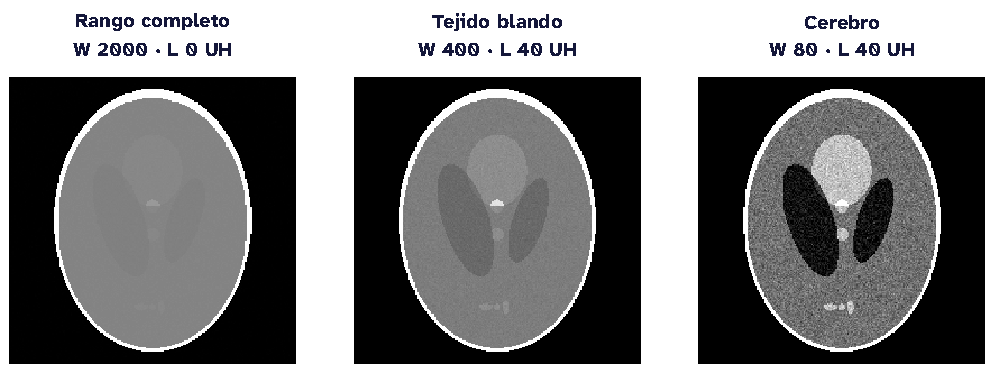
\includegraphics[width=0.9\linewidth,height=\textheight,keepaspectratio]{../fig/ventanas.pdf}

}

\caption{Tres ventanas sobre el mismo corte.}

\end{figure}%

Prueba al menos tres ventanas. Para cada una anota \(W\), \(L\) y qué
estructura se distingue mejor.

\begin{tcolorbox}[enhanced jigsaw, rightrule=.15mm, opacitybacktitle=0.6, colbacktitle=quarto-callout-warning-color!10!white, toptitle=1mm, opacityback=0, bottomrule=.15mm, title=\textcolor{quarto-callout-warning-color}{\faExclamationTriangle}\hspace{0.5em}{Cuidado}, leftrule=.75mm, colback=white, colframe=quarto-callout-warning-color-frame, coltitle=black, left=2mm, titlerule=0mm, bottomtitle=1mm, breakable, arc=.35mm, toprule=.15mm]

La ventana cambia la imagen que se muestra, no los datos. Las medidas
(áreas, intensidades) se hacen siempre sobre la matriz en UH.

\end{tcolorbox}

\section{Preguntas orientadoras}\label{preguntas-orientadoras}

\begin{enumerate}
\def\labelenumi{\arabic{enumi}.}
\tightlist
\item
  ¿Por qué el aire queda en −1000 UH y qué pasa con él en la ventana de
  cerebro?
\item
  Si el histograma tiene dos picos muy cercanos, ¿qué ventana los separa
  mejor y por qué?
\item
  ¿Qué información se pierde al guardar la imagen ya ventaneada en 8
  bits?
\end{enumerate}

\section{Entregables}\label{entregables}

\begin{itemize}
\tightlist
\item
  Un cuaderno o script reproducible con el histograma y las tres
  ventanas.
\item
  Una tabla con \(W\), \(L\) y la estructura que cada ventana deja ver.
\item
  Respuestas breves a las preguntas orientadoras.
\end{itemize}

\section{Rúbrica}\label{ruxfabrica}

\begin{longtable}[]{@{}
  >{\raggedright\arraybackslash}p{(\linewidth - 4\tabcolsep) * \real{0.3333}}
  >{\raggedleft\arraybackslash}p{(\linewidth - 4\tabcolsep) * \real{0.3333}}
  >{\raggedright\arraybackslash}p{(\linewidth - 4\tabcolsep) * \real{0.3333}}@{}}
\caption{Rúbrica del laboratorio 1.}\tabularnewline
\toprule\noalign{}
\begin{minipage}[b]{\linewidth}\raggedright
Criterio
\end{minipage} & \begin{minipage}[b]{\linewidth}\raggedleft
Peso
\end{minipage} & \begin{minipage}[b]{\linewidth}\raggedright
Logrado
\end{minipage} \\
\midrule\noalign{}
\endfirsthead
\toprule\noalign{}
\begin{minipage}[b]{\linewidth}\raggedright
Criterio
\end{minipage} & \begin{minipage}[b]{\linewidth}\raggedleft
Peso
\end{minipage} & \begin{minipage}[b]{\linewidth}\raggedright
Logrado
\end{minipage} \\
\midrule\noalign{}
\endhead
\bottomrule\noalign{}
\endlastfoot
Conversión y verificación del rango en UH & 25 \% & Explica los valores
extremos con las estructuras del fantoma \\
Histograma & 25 \% & Intervalos adecuados, ejes con unidades y picos
identificados \\
Elección de ventanas & 30 \% & Cada ventana se justifica con el
histograma \\
Reproducibilidad & 20 \% & El código corre de principio a fin sin pasos
manuales \\
\end{longtable}




\end{document}
